\documentclass[11pt,twoside]{article}
\usepackage{etex}

\usepackage{authblk}

\raggedbottom

\usepackage[eulergreek]{sansmath}

%\usepackage{natbib}

%geometry (sets margin) and other useful packages
\usepackage{geometry}
\geometry{top=1in, left=.9in,right=.9in,bottom=1in}
 \usepackage{graphicx,booktabs,calc}
\graphicspath{{./SI-Figures/}}
% Marginpar width
%Marginpar width
\newcommand{\pts}[1]{\marginpar{ \small\hspace{0pt} \textit{[#1]} } } 
\setlength{\marginparwidth}{.5in}
%\reversemarginpar
%\setlength{\marginparsep}{.02in}

\usepackage{morefloats}
%% Fonts
% \usepackage{fourier}
% \usepackage[T1]{pbsi}

\usepackage{lmodern}
\usepackage[T1]{fontenc}
%\usepackage{minted}

%% Cite Title
% \usepackage[style=numeric]{biblatex}
% \addbibresource{/Users/JimiOke/Dropbox/Research/references.bib}

%%% Counters
\usepackage{chngcntr,mathtools}
\counterwithout{figure}{section}
\counterwithout{table}{section}

\numberwithin{equation}{section}

\usepackage{tocloft}
\renewcommand{\cftfigpresnum}{S}
\renewcommand{\cfttabpresnum}{S}

%% Captions
\renewcommand{\figurename}{Fig.}

\usepackage[margin=.5in]{caption}
\DeclareCaptionLabelFormat{custom}{Supplementary #1 S#2}
\captionsetup{
  labelsep=quad,
  justification=raggedright,
  labelfont=bf,
  labelformat=custom,
  font=footnotesize
}

%AMS-TeX packages
\usepackage{amssymb,amsmath,amsthm} 
\usepackage{bm}
\usepackage[mathscr]{eucal}
\usepackage{colortbl}
\usepackage{color}



\usepackage{epstopdf,hyperref,enumerate,polynom,polynomial}
\usepackage{multirow,minitoc,fancybox,array,multicol}

\definecolor{slblue}{rgb}{0,.3,.62}
\hypersetup{
    colorlinks,%
    citecolor=blue,%
    filecolor=blue,%
    linkcolor=blue,
    urlcolor=slblue
}

%%%TIKZ
\usepackage{tikz}
\usepackage{pgfplots}
\usepackage{pgfplotstable} 
\usepackage{longtable}
\pgfplotstableset{
    col sep=comma,
    every head row/.style={before row=\toprule,after row=\midrule},
    every last row/.style={after row=\bottomrule}
    }

\pgfplotsset{compat=newest,
  tick label style = {font=\scriptsize},
  every axis label/.append style = {font=\footnotesize}}

\usetikzlibrary{arrows,shapes,positioning}
\usetikzlibrary{decorations.markings}
\usetikzlibrary{shadows,automata}
\usetikzlibrary{patterns}
%\usetikzlibrary{circuits.ee.IEC}
\usetikzlibrary{decorations.text}
% For Sagnac Picture
\usetikzlibrary{%
    decorations.pathreplacing,%
    decorations.pathmorphing%
}

\definecolor{strongred}{HTML}{D7191C}
\definecolor{softorange}{HTML}{FDAE61}
\definecolor{vslgreen}{HTML}{ABDDA4}
\definecolor{strongblue}{HTML}{2B83BA}


\usepackage{ctable}

\usepackage{paralist,pifont}
\newcommand{\cmark}{\ding{51}}%
\newcommand{\xmark}{\ding{55}}%

\newcommand{\osn}{\oldstylenums}
\newcommand{\dg}{^{\circ}}
\newcommand{\lt}{\left}
\newcommand{\rt}{\right}
\newcommand{\pt}{\phantom}
\newcommand{\tf}{\therefore}
\newcommand{\?}{\stackrel{?}{=}}
\newcommand{\fr}{\frac}
\newcommand{\dfr}{\dfrac}
\newcommand{\ul}{\underline}
\newcommand{\tn}{\tabularnewline}
\newcommand{\nl}{\newline}
\newcommand\relph[1]{\mathrel{\phantom{#1}}}
\newcommand{\cm}{\checkmark}
\newcommand{\ol}{\overline}
\newcommand{\rd}{\color{red}}
\newcommand{\bl}{\color{blue}}
\newcommand{\pl}{\color{purple}}
\newcommand{\og}{\color{orange!90!black}}
\newcommand{\gr}{\color{green!40!black}}
\newcommand{\nin}{\noindent}
\newcommand{\la}{\lambda}
\renewcommand{\th}{\theta}
\newcommand{\al}{\alpha}
\newcommand{\G}{\Gamma}
\newcommand*\circled[1]{\tikz[baseline=(char.base)]{
            \node[shape=circle,draw,thick,inner sep=1pt] (char) {\small #1};}}

\newcommand{\bc}{\begin{compactenum}[\quad--]}
\newcommand{\ec}{\end{compactenum}}

\newcommand{\p}{\partial}
\newcommand{\pd}[2]{\frac{\partial{#1}}{\partial{#2}}}
\newcommand{\dpd}[2]{\dfrac{\partial{#1}}{\partial{#2}}}
\newcommand{\pdd}[2]{\frac{\partial^2{#1}}{\partial{#2}^2}}

\newcommand{\zkr}{Z(k_{r})}
\newcommand{\zkb}{Z(k_{b})}
\newcommand{\zkl}{Z(k_{l})}
\newcommand{\ztot}{Z_{\mathrm{tot}}}
\newcommand{\alp}{\alpha_{\text{prec}}}
\newcommand{\alo}{\alpha_{\text{orig}}}
\newcommand{\als}{\alpha_{\text{succ}}}
\newcommand{\sepp}{\mathrm{sec}_{\text{prec}}}
\newcommand{\seo}{\mathrm{sec}_{\text{orig}}}
\newcommand{\ses}{\mathrm{sec}_{\text{succ}}}
\newcommand{\dir}{\mathrm{dir}}
\newcommand{\shi}{\mathrm{shift}}
\newcommand{\ben}{\mathrm{bend}}
\newcommand{\ali}{\alpha_{i}}
\newcommand{\nw}{N\"{o}llenburg and Wolff}
\newcommand{\linf}{L^{\infty}}
\newcommand{\incg}{\includegraphics}
\newcommand{\fns}{\footnotesize}
\newcommand{\scs}{\scriptsize}
%\newcommand{\tsb}{\textsubscript}
\newcommand{\mr}{\mathrm}
\allowdisplaybreaks



%Capitalize refs
%source: http://tex.stackexchange.com/a/40413/2269
\usepackage{catoptions}
\makeatletter
\def\figureautorefname{figure}
\def\tableautorefname{table}
\def\Autoref#1{%
  \begingroup
  \edef\reserved@a{\cpttrimspaces{#1}}%
  \ifcsndefTF{r@#1}{%
    \xaftercsname{\expandafter\testreftype\@fourthoffive}
      {r@\reserved@a}.\\{#1}%
  }{%
    \ref{#1}%
  }%
  \endgroup
}
\def\testreftype#1.#2\\#3{%
  \ifcsndefTF{#1autorefname}{%
    \def\reserved@a##1##2\@nil{%
      \uppercase{\def\ref@name{##1}}%
      \csn@edef{#1autorefname}{\ref@name##2}%
      \autoref{#3}%
    }%
    \reserved@a#1\@nil
  }{%
    \autoref{#3}%
  }%
}
\makeatother

%figure reference with letters

\newcommand{\figrefl}[2]{\hyperref[#1]{\Autoref{#1}#2}}
%For math sf:
\DeclareMathVersion{sansserif}
\SetSymbolFont{operators}{sansserif}{OT1}{cmss}{m}{n}



\setcounter{Maxaffil}{5}

%%%%%%%%%%%%%%%%%%%%%%%%%%%%%%%%%%%%%%%%%%%%%%%%%%%
%%%%%%%%%%%%%%%%%%%%%%%%%%%%%%%%%%%%%%%%%%%%%%%%%%%
\title{Supplementary Material for:\\
{\it Multimodal transportation flows in energy networks with an application
   to crude oil markets}}
\author[1,2,3,*]{Olufolajimi Oke}
\author[4,3,5]{Daniel Huppmann}
\author[1]{Max Marshall}
\author[1]{Ricky Poulton}
\author[1,3,6]{Sauleh Siddiqui}
\affil[1]{Department of Civil Engineering, The Johns Hopkins University, Baltimore, MD 21218, United States}
\affil[2]{Current Address: Department of Civil and Environmental Engineering, Massachusetts Institute of Technology, Cambridge, MA 02139, United States}
\affil[3]{Center for Systems Science and Engineering, The Johns Hopkins University, Baltimore, MD 21218,
  United States} 
\affil[4]{International Institute of Applied Systems Analysis (IIASA), 2361
  Laxenburg, Austria}
\affil[5]{German Institute for Economic Research (DIW Berlin), 10117 Berlin, Germany}
\affil[6]{Department of Applied Mathematics and Statistics, The Johns Hopkins University, Baltimore, MD 21218, United States}
\affil[*]{To whom correspondence should be addressed; E-mail: {oke@mit.edu}}
\renewcommand\Authands{ and }


\begin{document}
\maketitle


\abstract{In this supplement, we provide further information for the North
  American crude oil model (NACOM). This includes a complete list of nodes and
  arcs in the model (\Autoref{sec:nodes} and \Autoref{sec:arcs}), along with a
  brief background on the Petroleum Administration for Defense Districts (PADD)
  regional system in the United States (\Autoref{app:padd}).  We validate flow
  calibration for NACOM in \Autoref{app:calib}. The input data for NACOM, along
  with the Python scripts used in processing and illustrating, are available for
  download at \url{https://github.com/MODLJHU/nacom}.

%\eject
\tableofcontents
\bigskip
%\listoffigures
\bigskip
%\listoftables

\eject



\section{Data initialization recap}
We set 2012 as the base year for our model, which proceeds for two subsequent
periods in steps of 3 years, i.e.\ 2015 and 2018.  All quantities are expressed
in kilobarrel per day (kbpd) units. % For production,
% we assume a fixed greenhouse gas emission value of 0.12
% MMtCO\textsubscript{2}-e per unit.
An annual discount factor of 91\% and 95\% is applied to investment decisions
for producers and arc operators, respectively. Prices and all other monetary
values are in US dollar terms. 100\% capacity availability is assumed for all
producers (thus $\mr{avl}^{P} =1$ in all cases). An energy service efficiency of
98\% is assumed for all consumption nodes. We do not consider seasonal
variations in either production or consumption patterns. Details on our data are
provided in the following section.


\section{The Petroleum Administration for Defense Districts}
\label{app:padd}
\begin{figure}[h!]
  \centering
  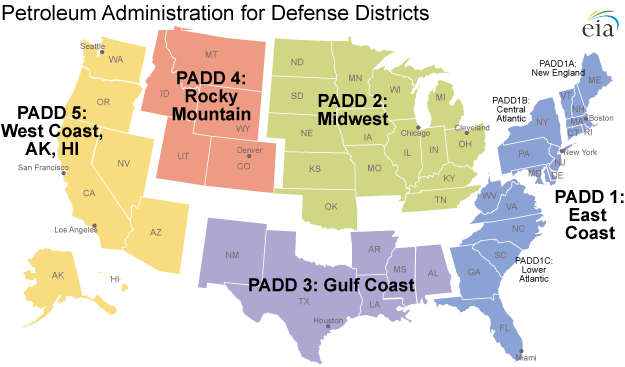
\includegraphics[width=4.5in]{PADDsMap}
  \caption[Petroleum Administration for Defense Districts]{Petroleum
      Administration for Defense Districts (Source: EIA \cite{eia2012padd})}
  \label{fig:padd}
\end{figure}

The Petroleum Administration Defense Districts (PADDs) were historically drawn
up to organize gasoline distribution during wartime rationing
\cite{eia2012padd}, but they have now been established as the baseline for
recording and analyzing crude oil movements in the US (\Autoref{fig:padd}),
especially by the US Energy Information Administration.  As described in
\Autoref{app:calib}, we use the PADD regional crude oil movement data as
the basis for calibrating base case flows through the US. We also occasionally
use them in highlighting regional changes at various points in this paper.


% \section{Flow maps}
% In 2015, there is heightened activity both within the pipeline and rail
% networks, as evidenced by the growth in production across the co
% \begin{figure}
%   \centering
%   \includegraphics[width=6in]{base_Rail_2015}
%   \caption{Rail flows of crude oil in 2015. The dashed green lines
%   indicate heavy crude, while the solid orange lines indicate light crude. The
%   thickness of the lines are varied according to the quantity
%   transported. Arrows along the tails of each arc show the direction of flow.}
%   \label{fig:base_Rail_2015}
% \end{figure}

% \begin{figure}
%   \centering
%   \includegraphics[width=6in]{base_Pipeline_2015}
%   \caption{Pipeline flows of crude oil in 2015. The dashed green lines
%   indicate heavy crude, while the solid orange lines indicate light crude. The
%   thickness of the lines are varied according to the quantity
%   transported. Arrows along the tails of each arc show the direction of flow.}
%   \label{fig:base_Pipeline_2015}
% \end{figure}




%}

% \subsection{Estimating U.S. refinery yields for light-sweet crude}

% Each region's mean API value was divided by the cutoff point from heavy to light


\section{List of nodes}
\label{sec:nodes}
\Autoref{tab:nodes} lists the nodes in the model, their abbreviations and their
regions.

{\footnotesize
  \pgfplotstableset{
    begin table=\begin{longtable},
      end table=\end{longtable}
  }
    \pgfplotstabletypeset[
      %header=true,
      columns={Node, Abbreviation, Region, Producer, Consumer},  
      columns/Node/.style={column type={l},string type},
      columns/Abbreviation/.style={column type={l},string type,
          postproc cell content/.code={%
            \pgfplotsutilstrreplace{_}{\_}{##1}%
            \pgfkeyslet{/pgfplots/table/@cell content}\pgfplotsretval
          }},
      columns/Region/.style={column type={l},string type},
      columns/Producer/.style={column type={l},int detect},
      columns/Consumer/.style={column type={l},int detect},
      every head row/.style={
       before row={\caption[]{List of nodes, their abbreviations and regions in
           the model. A value of 1 or 0 indicates whether the node is a
           producing/consuming node or not.}  
         \label{tab:nodes} \\\toprule 
         },
         after row={\midrule\endfirsthead}
       },
    every last row/.style={after row=\bottomrule},
    every head row/.append style={
       before row={\caption[]{List of nodes, their abbreviations and regions in
           the model. A value of 1 or 0 indicates whether the node is a
           producing/consuming node or not.} 
         \label{tab:nodes} \\\toprule
         },
         after row={\midrule\endhead}}
      ]{nodenames.csv}     
}



\section{Transportation arcs in the model and their initial parameter values}
\label{sec:arcs}
The arc data gathered for the model are shown in \Autoref{tab:arcs}. Some
parameters were later adjusted for calibration purposes.
{\footnotesize
  \pgfplotstableset{
    begin table=\begin{longtable},
      end table=\end{longtable}
  }
    \pgfplotstabletypeset[
      %header=true,
      columns={Outgoing Node, Incoming Node, Type, Tariff, Capacity, Capacity Constrained},  
      columns/Outgoing Node/.style={column type={l},string type, 
        postproc cell content/.code={%
          \pgfplotsutilstrreplace{_}{\_}{##1}%
          \pgfkeyslet{/pgfplots/table/@cell content}\pgfplotsretval
        }},
      columns/Incoming Node/.style={column type={l},string type,
          postproc cell content/.code={%
            \pgfplotsutilstrreplace{_}{\_}{##1}%
            \pgfkeyslet{/pgfplots/table/@cell content}\pgfplotsretval
          }},
      columns/Type/.style={column type={l},string type},
      columns/Tariff/.style={column type={l},fixed,precision=2},
      columns/Capacity/.style={column type={l},fixed,precision=2},
      columns/Capacity Constrained/.style={column type={l},int detect},
     every head row/.style={
       before row={\caption[Transportation arcs for crude oil included in the
         model]{Transportation arcs for crude oil included in the
         model. Capacities shown are initial values, some of which are modified
         in calibration. The term ``BargeS'' represents sea-going barges, while
         ``BargeR'' represents river-going barges. A value of 1 for the
         ``Capacity Constrained'' parameter indicates that the capacity is
         active. Most of the waterway arcs were initialized with unlimited (or
         unconstrained) capacities, but limits were introduced during
         calibration. All tariff values are in US\$/barrel.}  
         \label{tab:arcs} \\\toprule 
         },
         after row={\midrule\endfirsthead}
       },
    every last row/.style={after row=\bottomrule},
    every head row/.append style={
       before row={\caption[]{Transportation arcs for crude oil included in the
         model. Capacities shown are initial values, some of which are modified
         in calibration. The term ``BargeS'' represents sea-going barges, while
         ``BargeR'' represents river-going barges. A value of 1 for the
         ``Capacity Constrained'' parameter indicates that the capacity is
         active. Most of the waterway arcs were initialized with unlimited (or
         unconstrained) capacities, but limits were introduced during
         calibration. All tariff values are in US\$/barrel.} 
         \label{tab:arcs} \\\toprule
         },
         after row={\midrule\endhead}}
      ]{Arcs.csv}     
}

\eject

\section{Model and reference flow comparisons}
\label{app:calib}

To validate our model, we compare equilibrium transportation quantities to
reference data at the regional level, which is the best resolution
available. The interregional flows in the base year 2012 for each of the modes
are shown in \Autoref{fig:calrail_12}, \Autoref{fig:calpipe_12} and
\Autoref{fig:calship_12}.

\bigskip

\begin{figure}[h!]
  \centering
  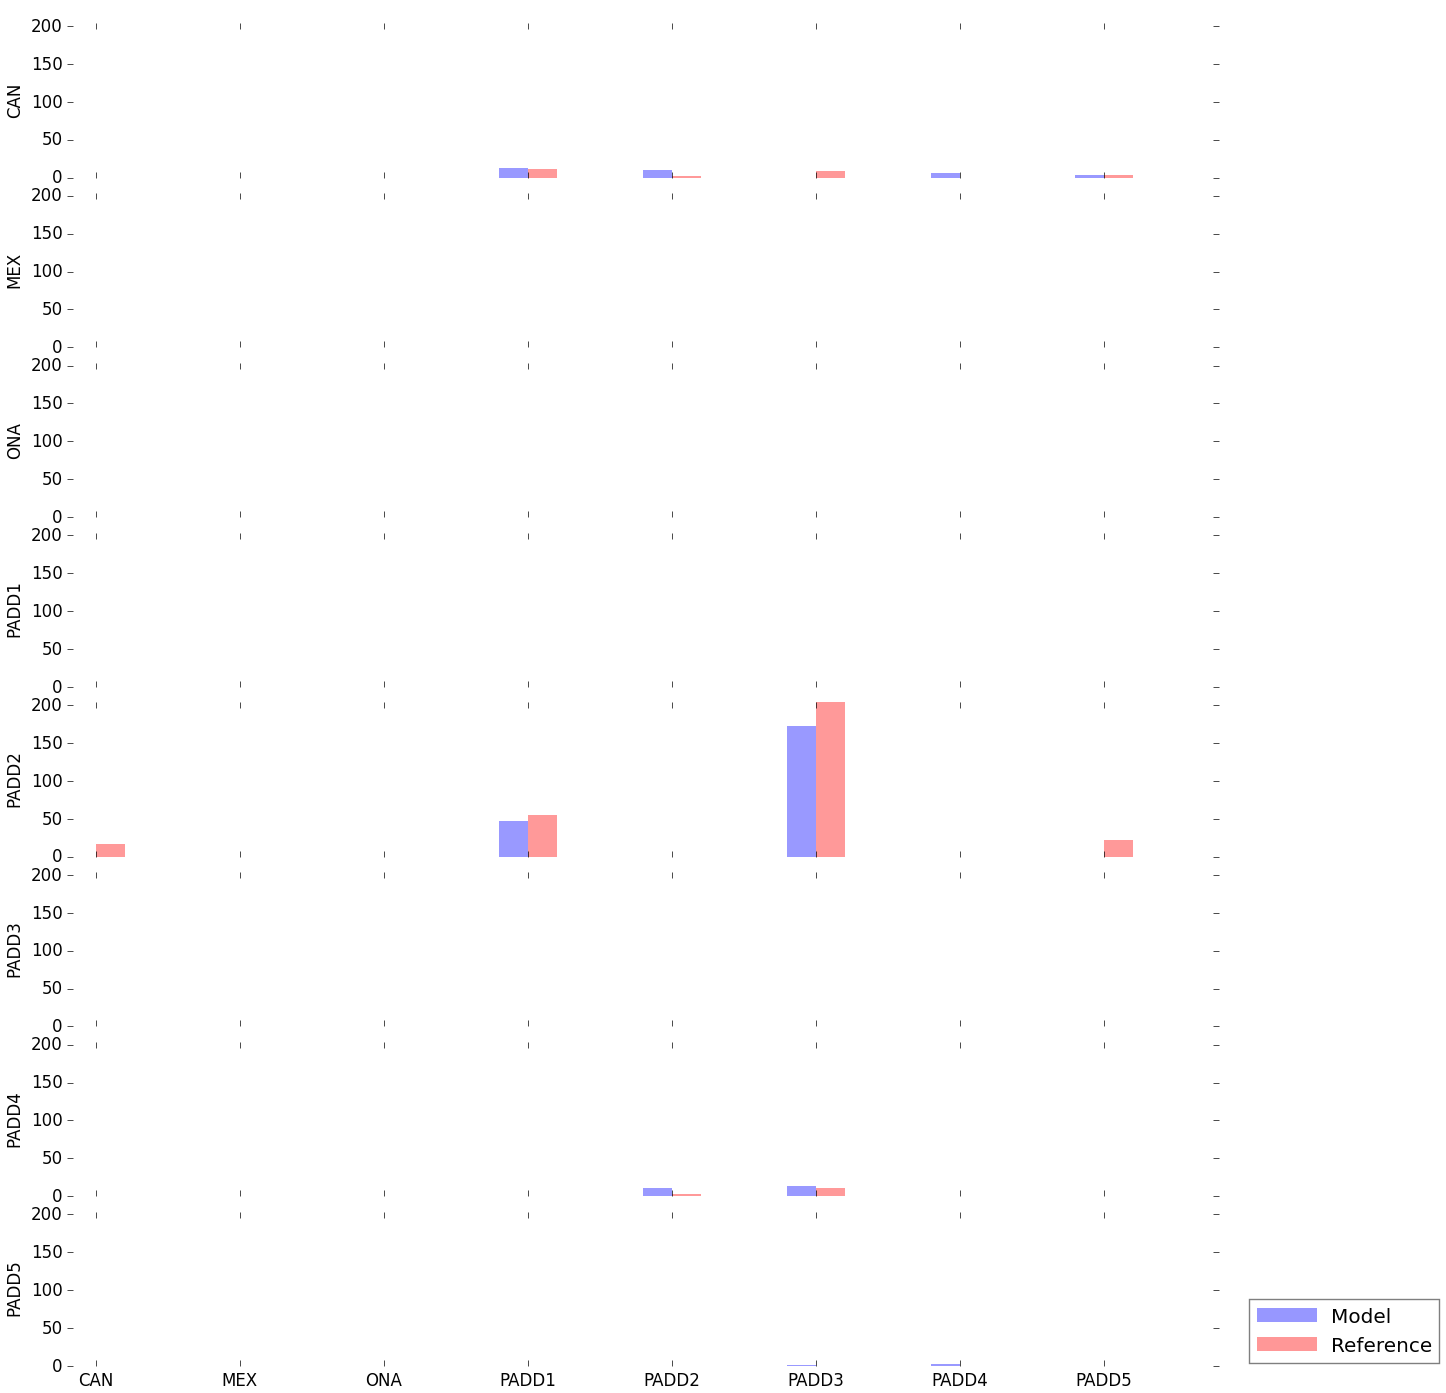
\includegraphics[width=\textwidth]{calibRail2012}
  \caption{Comparison of model and reference interregional transportation
    quantities via rail in 2012}
  \label{fig:calrail_12}
\end{figure}

\eject

\begin{figure}[h!]
  \centering
  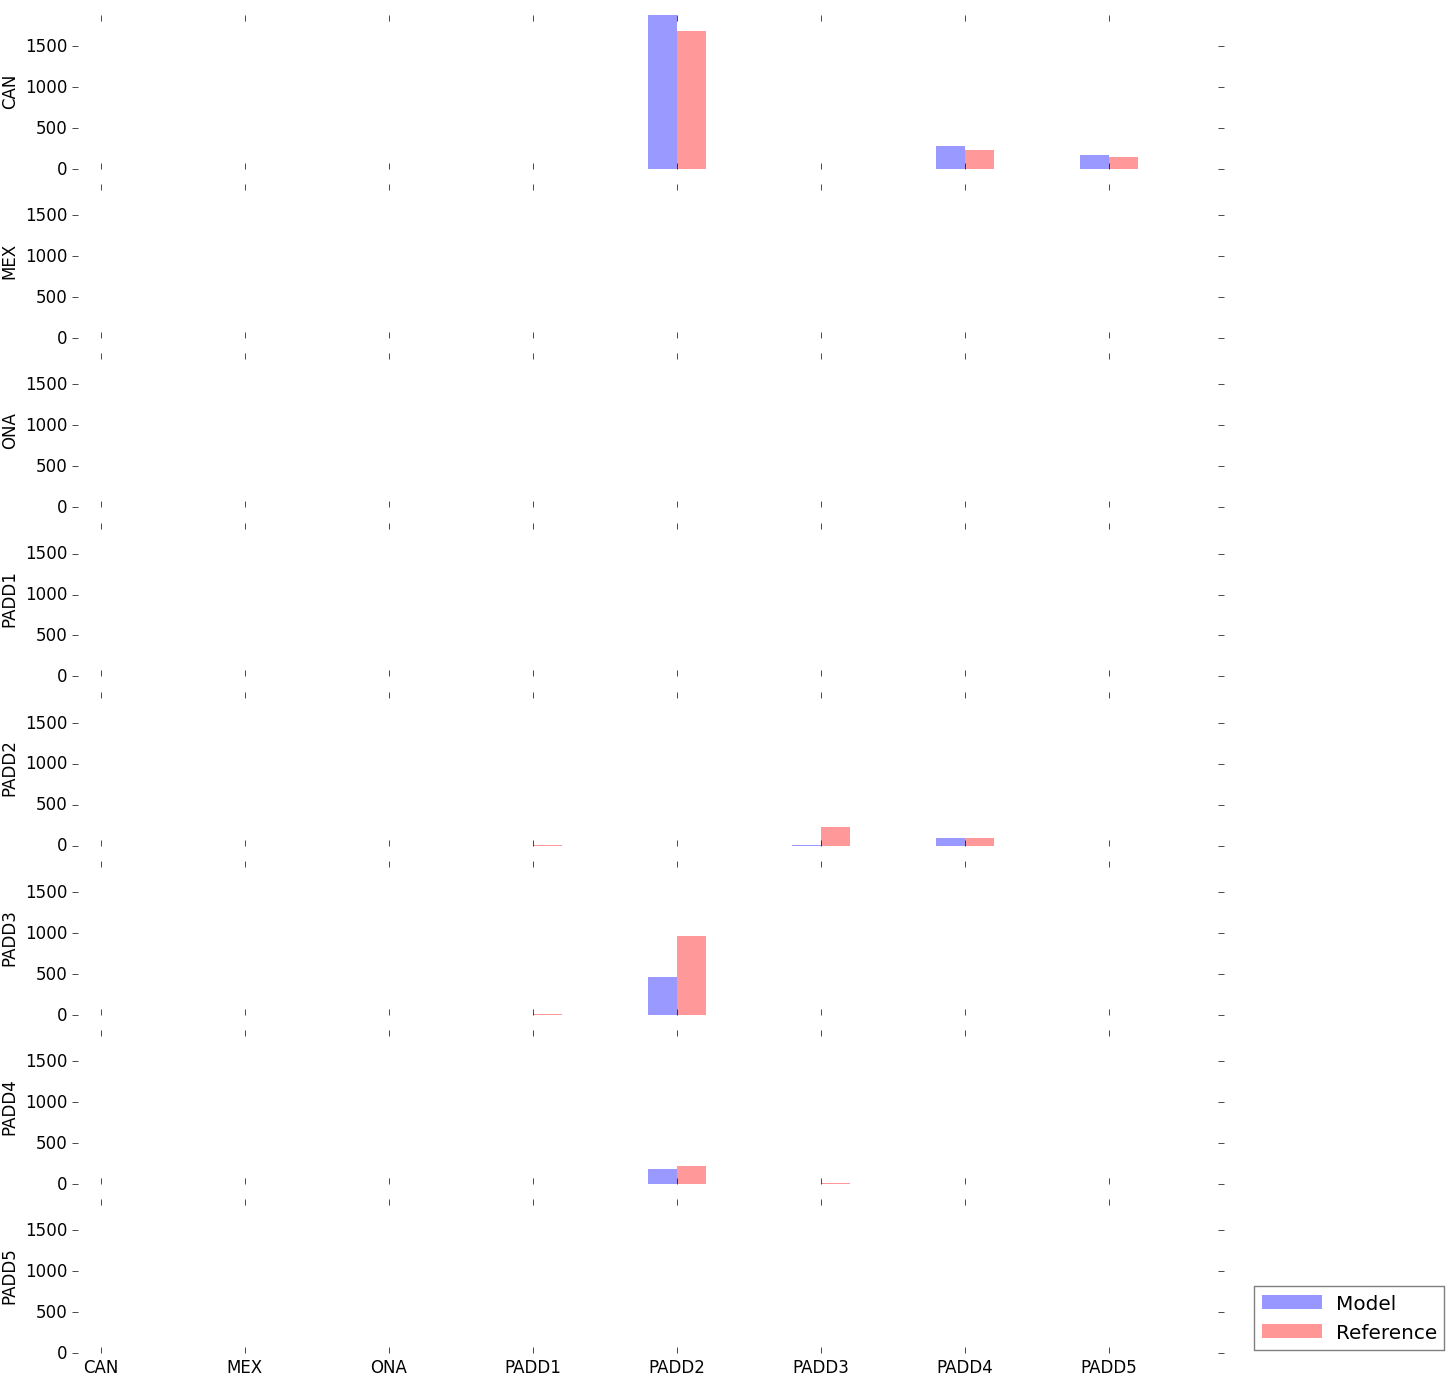
\includegraphics[width=\textwidth]{calibPipe2012}
  \caption{Comparison of model and reference interregional transportation
    quantities via pipeline in 2012}
  \label{fig:calpipe_12}
\end{figure}

\eject

\begin{figure}[h!]
  \centering
  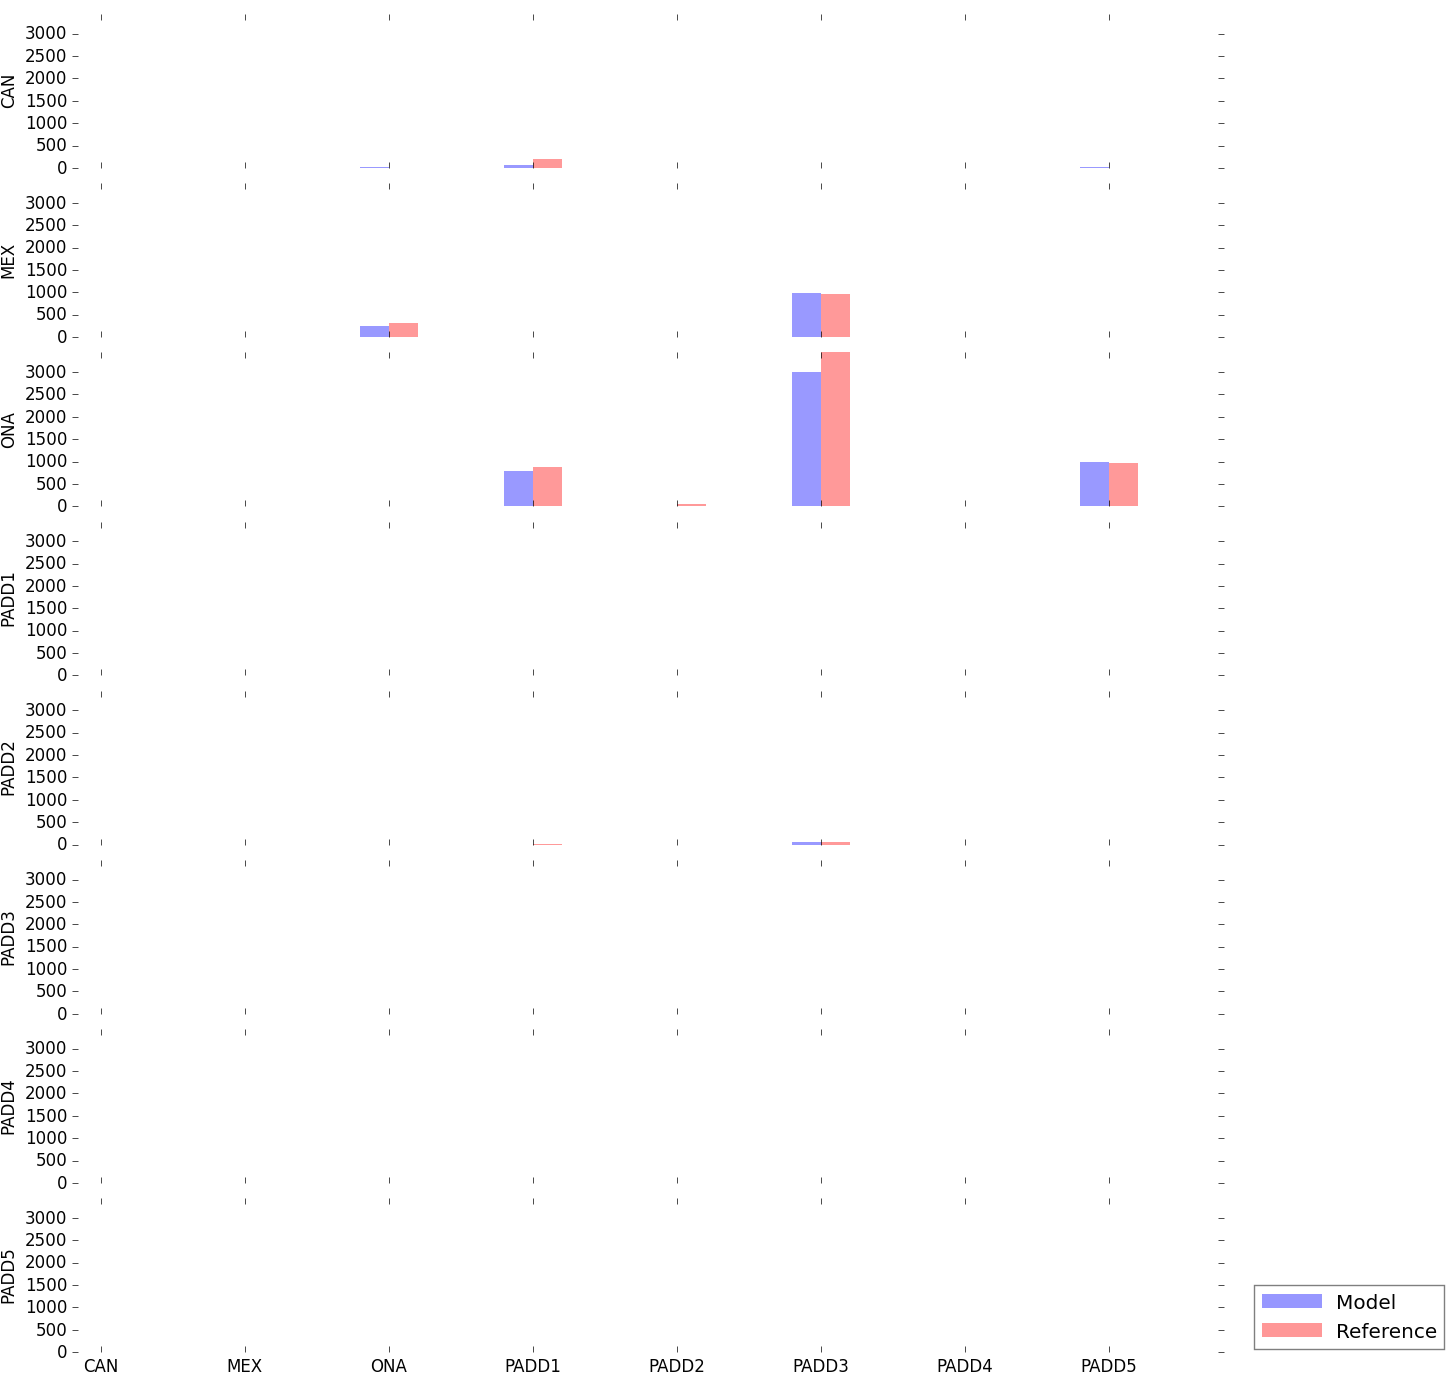
\includegraphics[width=\textwidth]{calibShip2012}
  \caption{Comparison of model and reference interregional transportation
    quantities via tanker/barge in 2012}
  \label{fig:calship_12}
\end{figure}

\eject

\subsection*{Note on figures}
All the figures in the main article and this supplement were created using the
Matplotlib package in Python \cite{hunt07} (except for Figure 1, which was
generated in \LaTeX via the {\sc pgf} package).


\bibliographystyle{plain}
\bibliography{../OOT-references.bib}
%\appendix

\end{document}